% 2009 年湖南卷理科第 4 题：函数 y=x/(1+λx)（x≥0）的两条曲线 C1、C2。
% 来源 PDF：普通高考/2009/2009湖南理.pdf，SHA-256 0237bd2509e6645937e3473eabb63dba69098024fb6f451cb44ef8ac0e3165c1。
% 原页：第 1 页（A3 三栏）第 1 栏中部，书页码 527。
% 重绘依据：曲线按 λ1>λ2>0 绘制（λ2=0.45、λ1=1.2），上方为 C2；只画第一象限，
%   与原页一致保留坐标轴箭头、原点 O 及 C1、C2 两个标注。
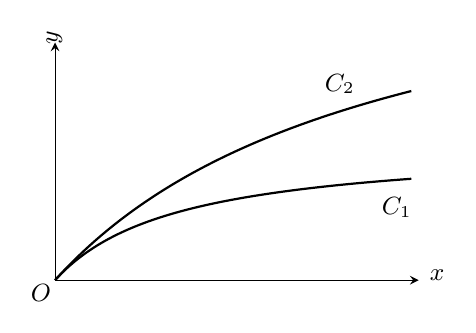
\begin{tikzpicture}[semithick, every node/.style={inner sep=1.2pt, font=\small}]
  \begin{axis}[
    width=6.2cm, height=4.6cm,
    axis lines=left,
    xmin=0, xmax=2.45, ymin=0, ymax=1.45,
    xtick=\empty, ytick=\empty,
    xlabel={$x$}, ylabel={$y$},
    xlabel style={at={(axis description cs:1.02,0.02)}, anchor=west},
    ylabel style={at={(axis description cs:0.03,1.02)}, anchor=south},
    axis line style={-stealth},
    clip=false,
  ]
    \addplot[domain=0:2.4, samples=120, thick] {x/(1+1.2*x)} node[pos=0.88, below right=4pt] {$C_1$};
    \addplot[domain=0:2.4, samples=120, thick] {x/(1+0.45*x)} node[pos=0.88, above left=2pt] {$C_2$};
    \node[below left] at (axis cs:0,0) {$O$};
  \end{axis}
\end{tikzpicture}
